% ===== Wrap-up (slides 104-113) =====
\sectionframe{Summary}

\begin{frame}{Summary}
  \begin{itemize}
    \item What \textbf{Kubernetes} is and why it is the backbone of modern infrastructure
    \item Manifests - the declarative way to define your cluster's desired state
    \item Building Blocks of a \textbf{Cluster}
      \begin{itemize}
        \item Pods - the smallest deployable units
        \item Deployments - manage replicas and rolling updates
        \item Services - stable endpoints for dynamic workloads
        \item Ingresses - routing external traffic into the cluster
      \end{itemize}
    \item Namespaces - organize and control environments and teams cleanly
    \item \textbf{Helm} - the package manager for Kubernetes
  \end{itemize}
\end{frame}

\begin{frame}{Summary}
  \begin{itemize}
    \item What we achieved today:
      \begin{itemize}\item You deployed the Pedelec server project to the cloud!\end{itemize}
  \end{itemize}
  \vfill\centering\removedimage{``not bad'' reaction meme}\vfill
  \emph{..but where to go from here?}
\end{frame}

\begin{frame}{Further Materials and Topics}
  \begin{columns}[T]
    \column{0.5\textwidth}
      \textbf{Developer side}
      \begin{itemize}
        \item Make it big: \textbf{Autoscalers}
        \item ENV variables: \textbf{ConfigMaps} and \textbf{Secrets}
        \item Deep Dive: \textbf{Labels} and \textbf{LabelSelectors}
        \item Persistent Storage: \textbf{Volumes} and \textbf{VolumeClaims}
      \end{itemize}
    \column{0.5\textwidth}
      \textbf{Kubernetes Internals}
      \begin{itemize}
        \item Cluster Architecture
        \item Control Plane
        \item Container Lifecycle
        \item CRI, CNI, CSI
      \end{itemize}
  \end{columns}
\end{frame}

\begin{frame}{Resources}
  \begin{itemize}
    \item Docker
      \begin{itemize}
        \item \url{https://docs.docker.com/compose/}
        \item \url{https://docs.docker.com/compose/compose-file/}
      \end{itemize}
    \item Kubernetes
      \begin{itemize}\item \url{https://kubernetes.io/docs}\end{itemize}
  \end{itemize}
  \bigskip
  All materials, exercises, and this deck:\\
  \url{https://github.com/Mtze/kubernetes-workshop}
  \bigskip

  Presented by \textbf{\wsPresenter}.
\end{frame}

\sectionframe{[Optional] Kubernetes under the hood}

\begin{frame}{Control Plane}
  \centering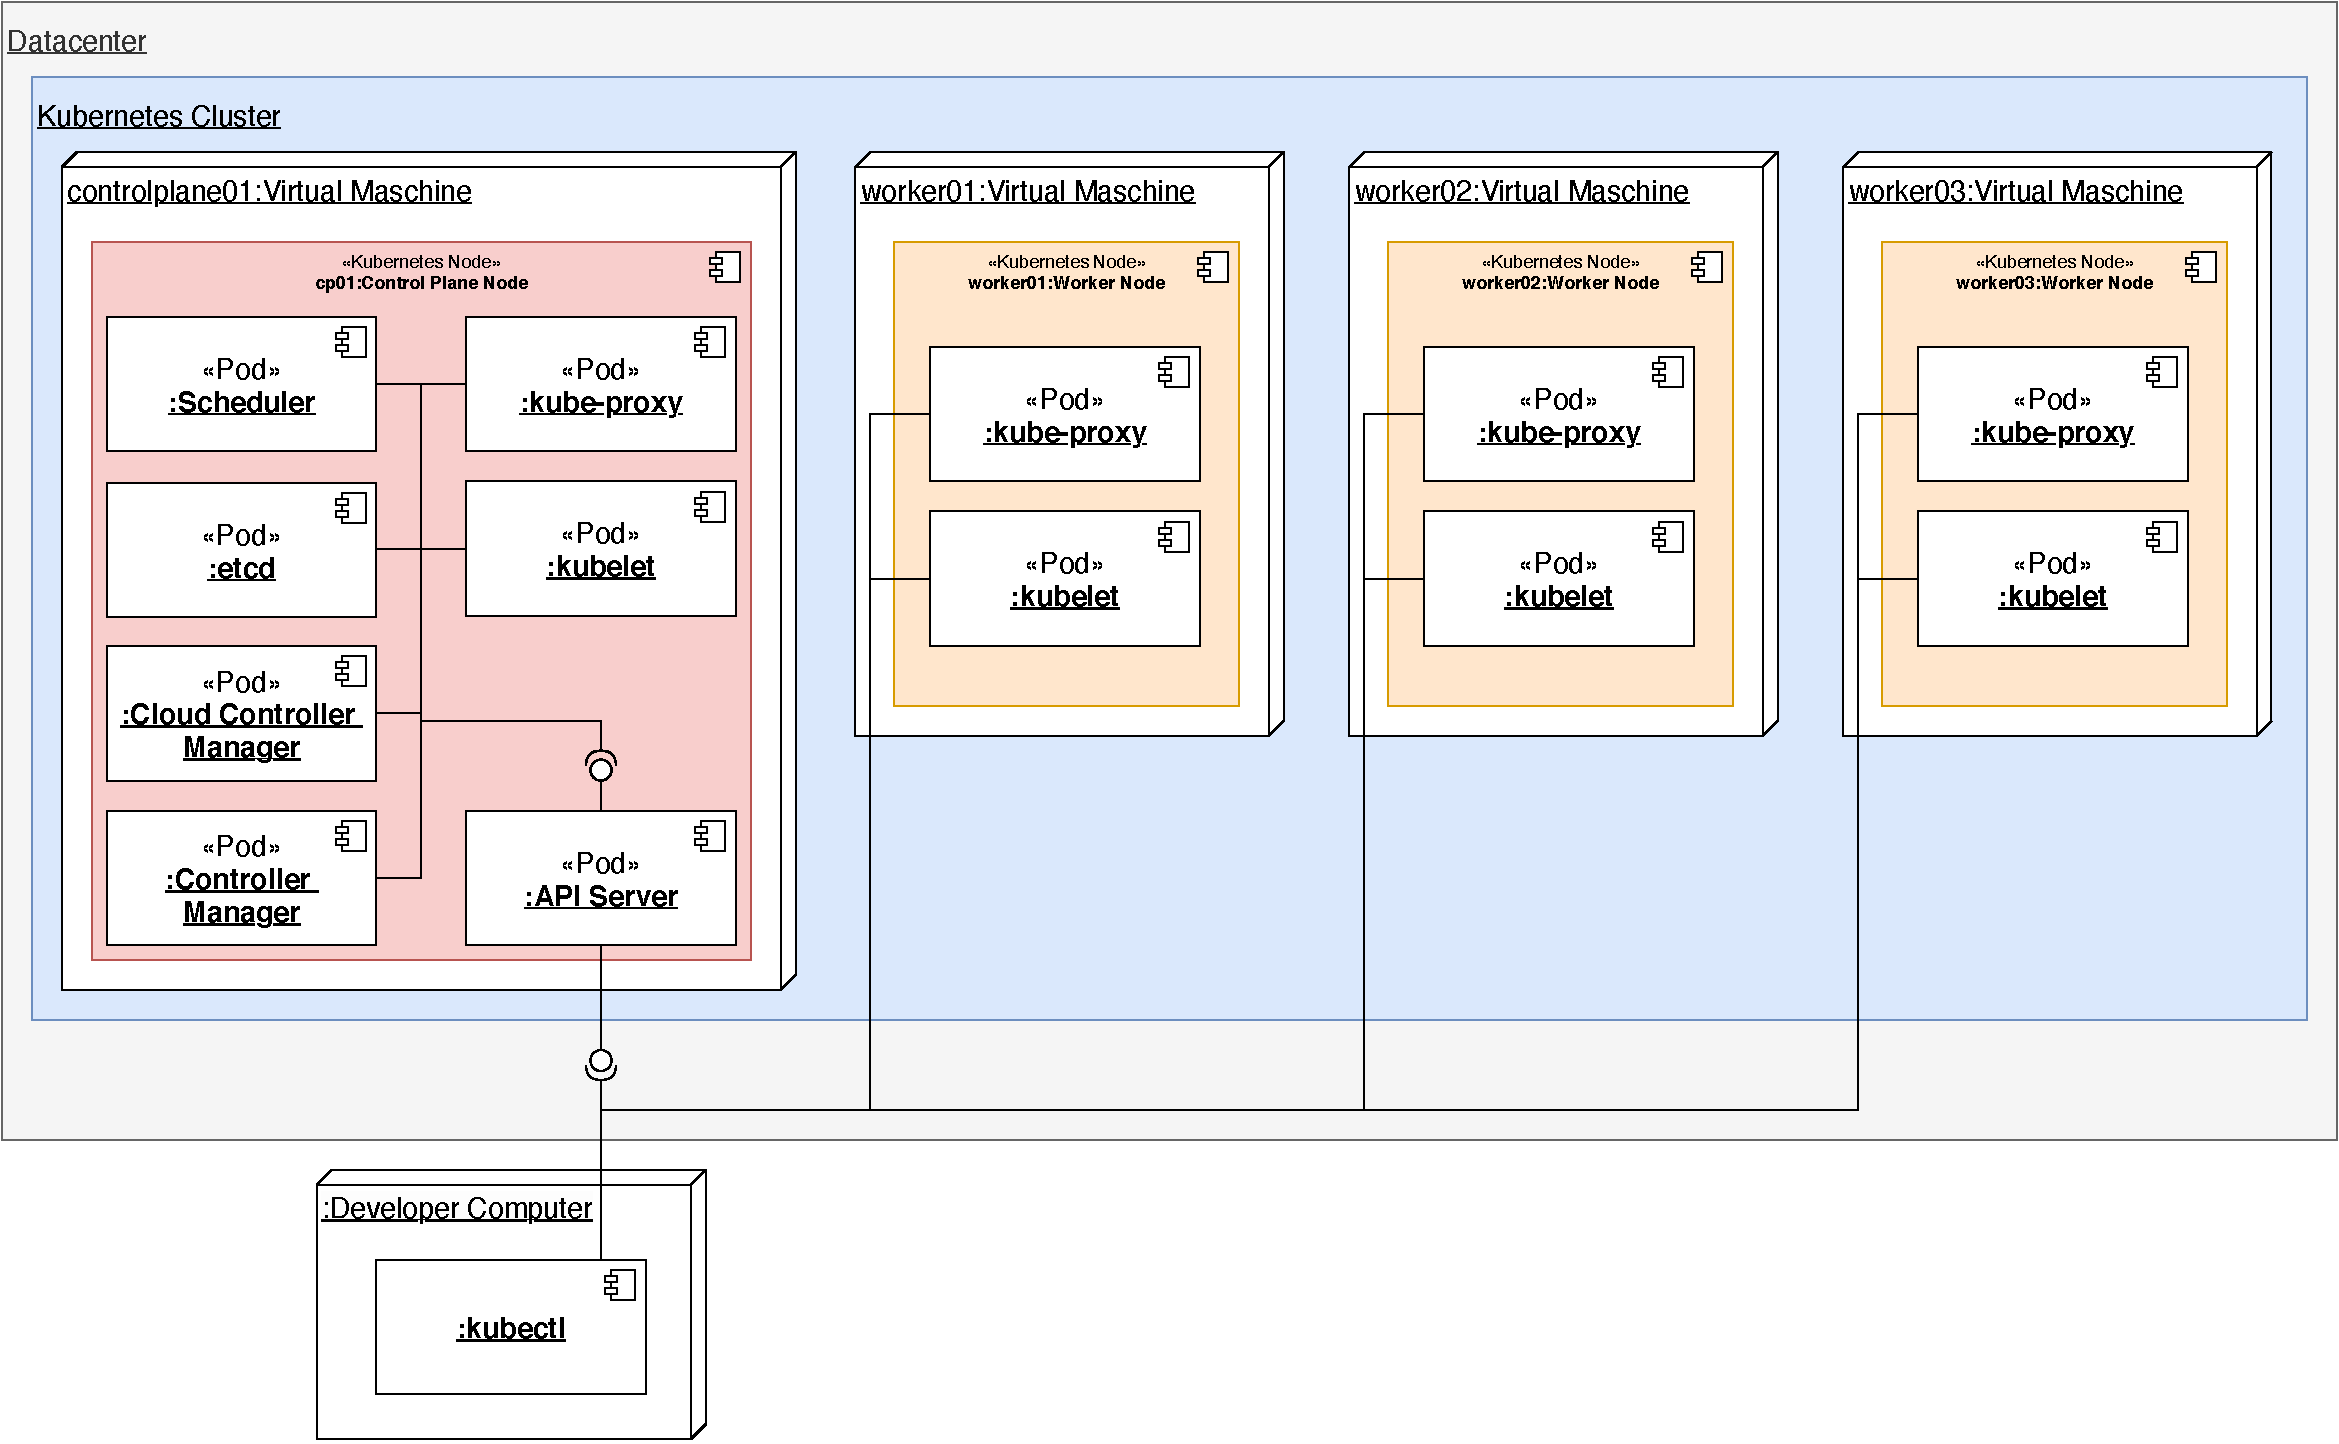
\includegraphics[height=0.74\paperheight]{assets/dia-component.pdf}
\end{frame}

\begin{frame}{Kubernetes Networking}
  \centering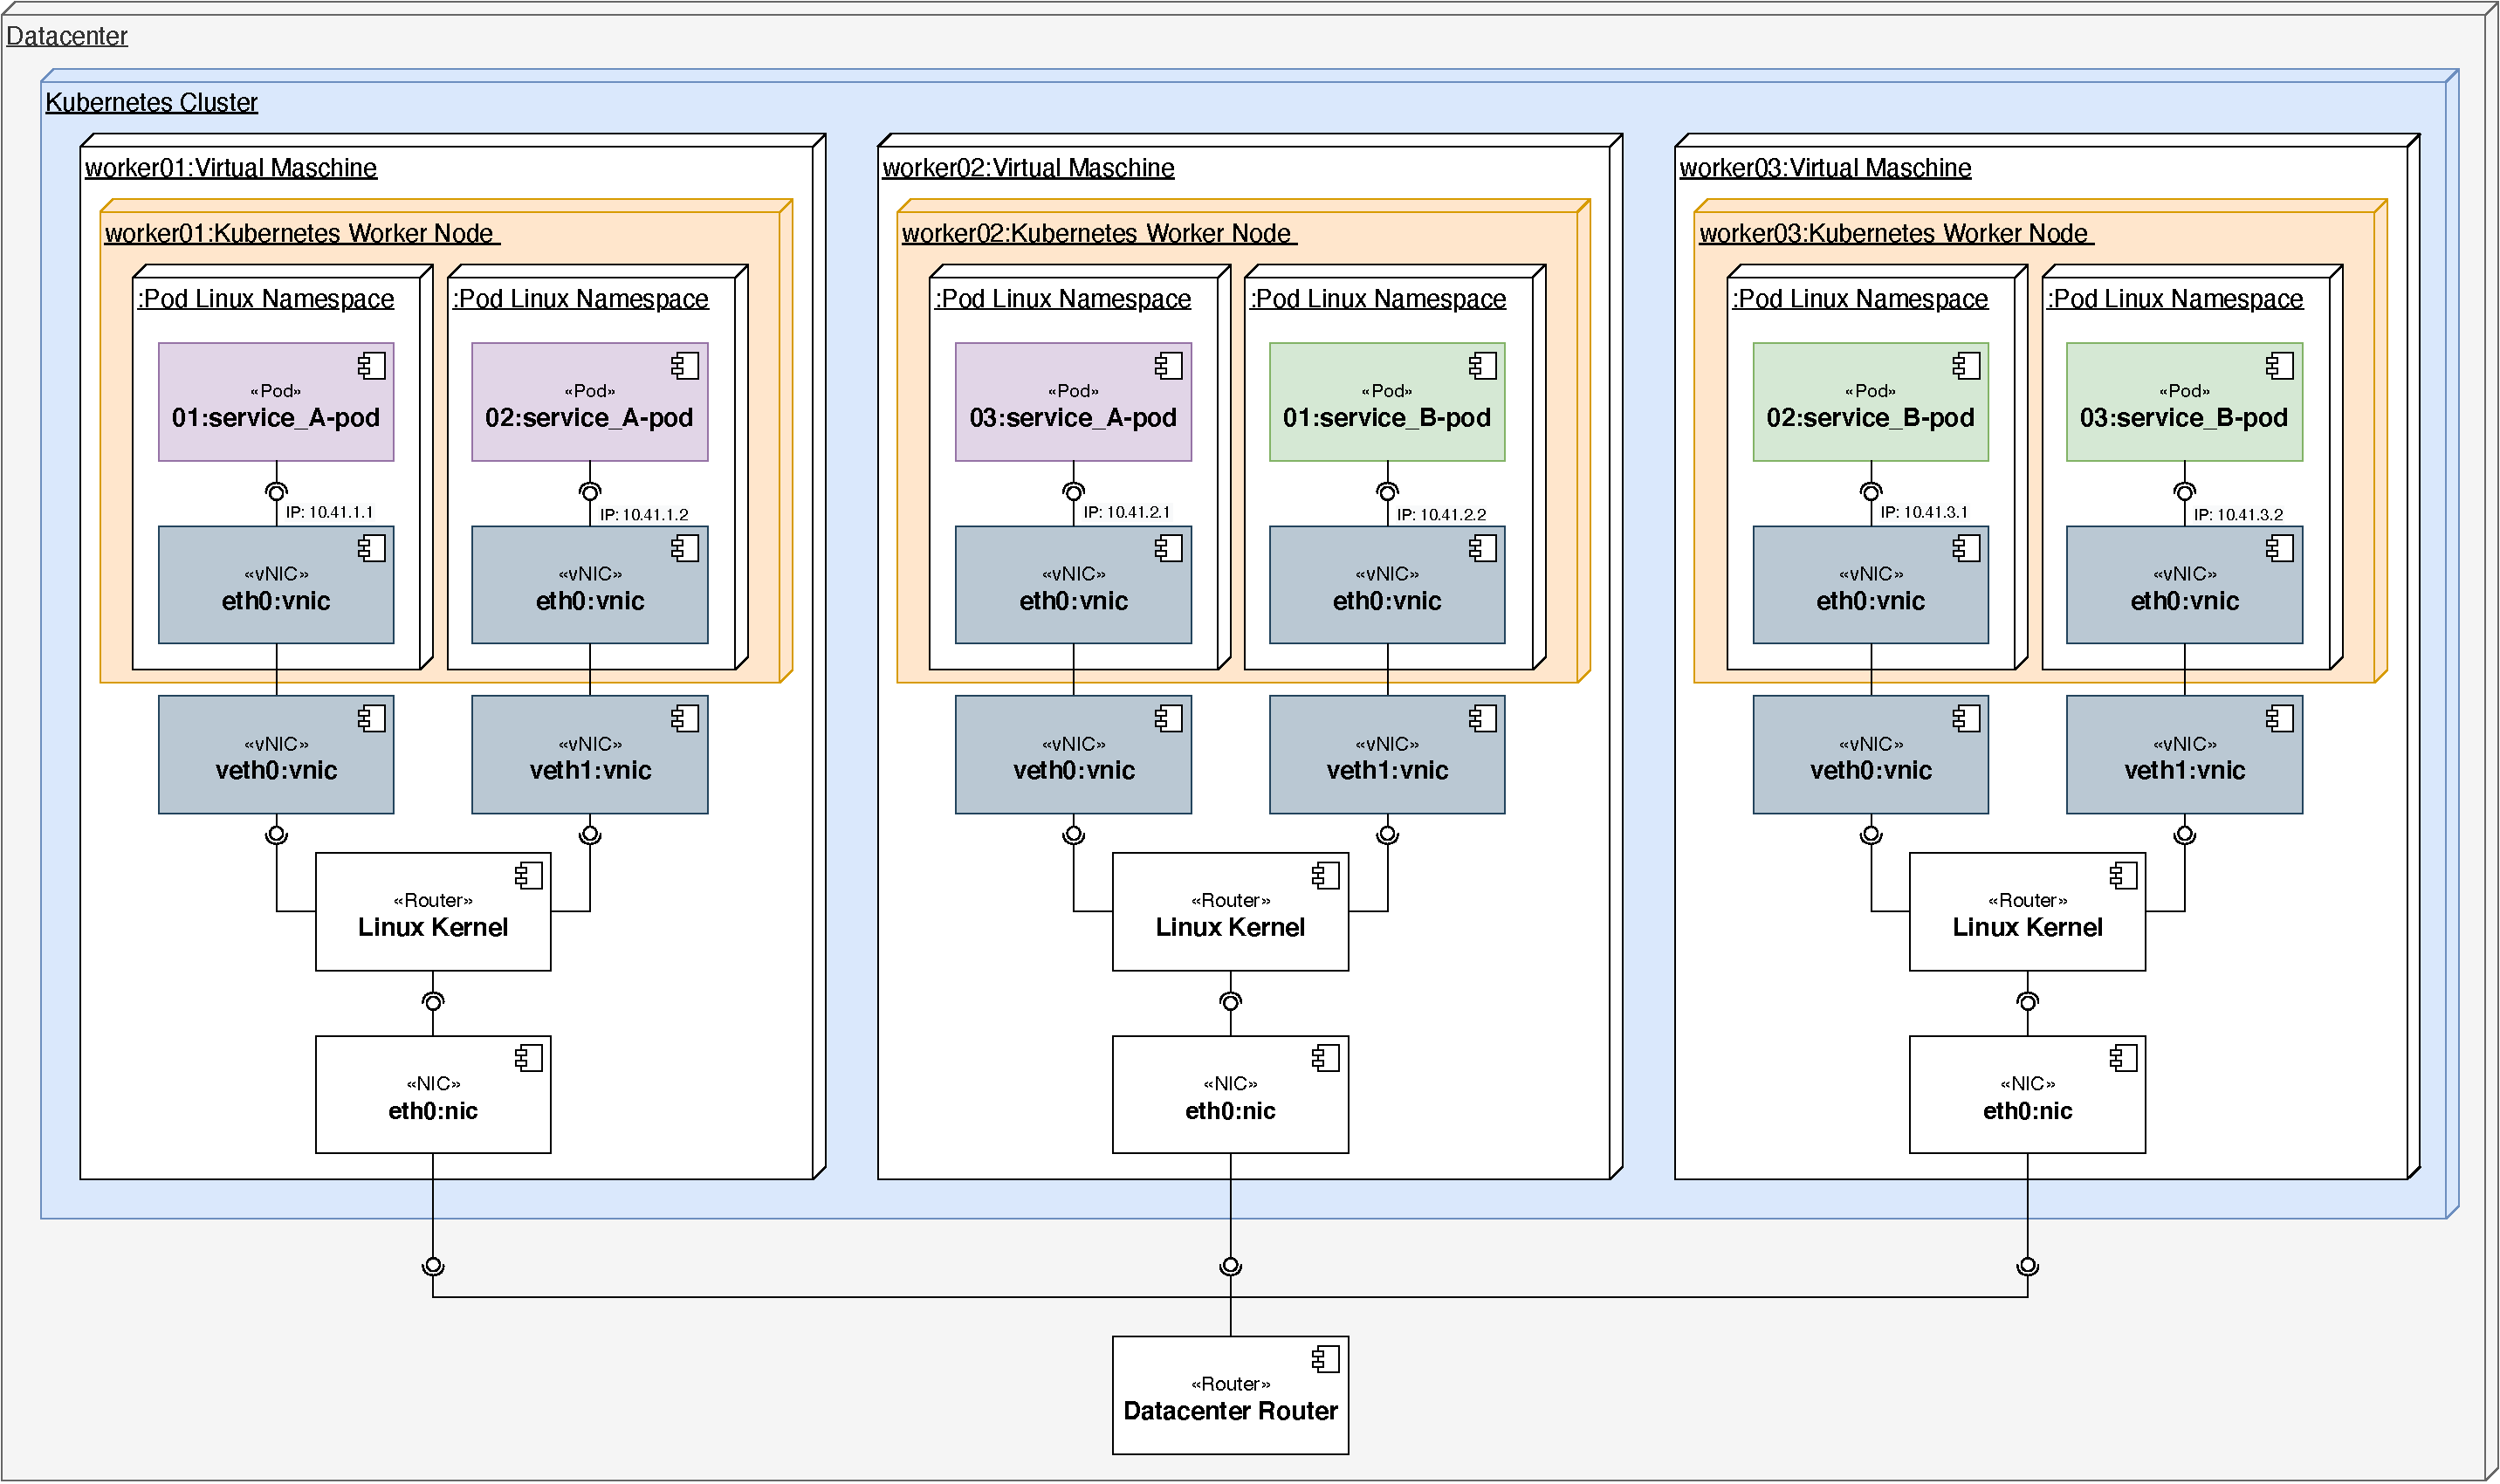
\includegraphics[width=\textwidth,height=0.74\paperheight,keepaspectratio]{assets/dia-component-annotated.pdf}
\end{frame}

\begin{frame}{Kubernetes Storage}
  \centering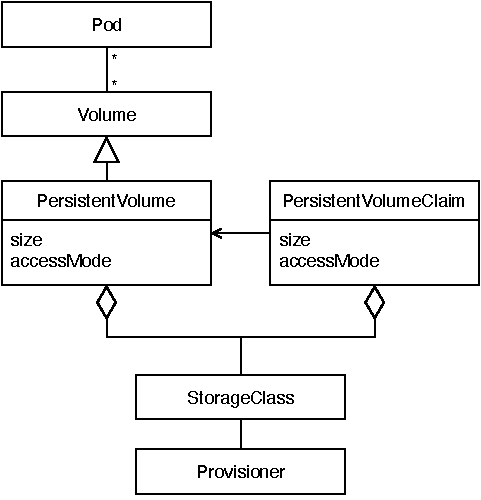
\includegraphics[height=0.74\paperheight]{assets/dia-storage.pdf}
\end{frame}
